\section{Analisi della macchina}
\subsection{Introduzione}
I compressori alternativi possono essere caratterizzati tramite diversi diagrammi (T-s, p-V, h-s), il più interessante per l'applicazione in esame è il diagramma indicato p-V. \\
\\
Il diagramma indicato è un diagramma che ha la pressione in ordinata e il volume in ascissa.
Non è un diagramma termodinamico, perché il volume in ascissa non è il volume specifico del fluido, ma è il volume (in $m^3$) del cilindro spazzato dal pistone durante il suo funzionamento. (Non si definisce in maniera univoca lo stato termodinamico del fluido).\\
Questo diagramma spiega semplicemente come cambia la pressione all’interno della macchina. 
\paragraph{Caso ideale}Il diagramma è compreso tra un volume minimo (stantuffo in PME) e un volume massimo (stantuffo in PMI), tra PME e PMI si identifica la cilindrata, ovvero il volume spazzato dal pistone. \\
\begin{figure}[h]
    \centering
    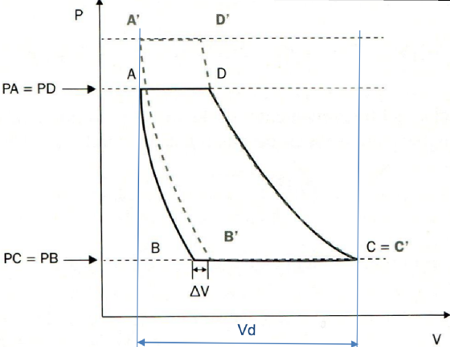
\includegraphics{Immagini/CasoIdeale.png}
    \caption{Andamento diagramma p-V caso ideale}
    \label{fig:CasoIdeale}
\end{figure}
\\
Nel punto di fine aspirazione C, inizia la compressione, il volume a disposizione del fluido inizia a ridursi e la pressione inizia ad aumentare, fino a quando la pressione all’interno del cilindro diventa uguale (caso ideale) alla pressione esterna, cioè quella all'interno del condotto di mandata.  Si arriva così al punto D, dove la pressione all’interno del cilindro è uguale alla pressione all’esterno, la valvola automatica si apre istantaneamente e avviene il trasferimento del fluido da dentro al cilindro alla mandata (non cambiano le caratteristiche del fluido perché non si ha più lo stantuffo che lo comprime, semplicemente viene spinto fuori dal pistone, su un diagramma T-s il tratto DA sarebbe un punto, perché non avviene una trasformazione termodinamica). \\
Si arriva dunque al punto A, lo stantuffo inverte la corsa, il volume a disposizione comincia ad aumentare, la pressione inizia a diminuire (espansione del gas rimanente dentro il cilindro) e la valvola di mandata si chiude immediatamente. Quando la pressione all'interno del cilindro diventa uguale a quella di aspirazione, la valvola si apre e il tratto di  corsa da B verso C vede il gas entrare dentro il cilindro (anche in questo caso nel piano T-s il punto B coincide con C). \\
\\
Ci sono caratteristiche di questo diagramma che dipendono dalla geometria del compressore (volume minimo e cilindrata) e altre caratteristiche che non dipendono prettamente dalla macchina, ma dipendono da come questa sta lavorando.\\
\\
Se la pressione di mandata diventa più alta (D’ e A’), il diagramma indicato cambia a parità di compressore. Si deve raggiungere una pressione più elevata rispetto a prima per aprire la valvola. Essendo la pressione più elevata, serve una corsa più lunga per diminuirla fino al livello di prima e quindi l’aspirazione inizia dopo. 
Come risultato finale si ottiene la riduzione della corsa per l’aspirazione all’aumentare della pressione di mandata. All’aumentare della pressione di mandata si riducono sempre di più i tratti orizzontali del diagramma. (Se si ha una pressione di mandata così elevata che tutta la corsa utile del pistone non riesce a creare una depressione tale da aprire le valvole, il compressore diventa una molla pneumatica). \\
Ha senso quindi utilizzare il compressore per un certo valore della pressione di mandata. \\
\\
Si traducono questi concetti in equazioni.\\
\\
Si definisce il coefficiente di volume ideale come:
\begin{equation}
 \lambda_{Vi}=\frac{m_C-m_B}{\rho_{AS}\cdot V_d}=\frac{\mbox{massa aspirata}}{\mbox{massa ideale, massimo fluido che si può introdurre nel cilindro}}.
\end{equation}
La portata massica ideale la si può esprimere come portata massica aspirabile corretta dal coefficiente volumetrico ideale, moltiplicata per i giri al secondo $\dot{m}=\lambda_{Vi}\cdot\rho_{AS}\cdot\ V_d\cdot\frac{n}{60}\ .$\\
\\
Si definisce coefficiente di volume nocivo come:  $\varepsilon=\frac{V_A}{V_d}$ .\\
\\
Il rapporto tra la pressione di mandata e la pressione di aspirazione viene chiamato rapporto di compressione $\frac{V_B}{V_A}=\left(\frac{p_B}{p_A}\right)^\frac{1}{k}=\beta^\frac{1}{K}$. Si ottiene quindi $\lambda_{Vi}=1-\varepsilon\left(\beta^{1/k}-1\right)$.\\
\\
All’aumentare di $\beta$, $\lambda_{Vi}$ diminuisce, che è esattamente quello che si è detto prima commentando il diagramma indicato. La massa di aria aspirata diminuisce all’aumentare della pressione di mandata e quindi del $\beta$ (tenendo implicitamente costante la pressione di aspirazione). Ne consegue che più grande è il volume minimo, più grande è $\varepsilon$ (a parità di cilindrata), il quale essendo negativo fa diminuire il $\lambda_{Vi}$ a parità di $\beta$, da qui il termine nocivo (perché minore è la portata che il compressore può erogare). \\
Chiaramente più è grande il volume minimo, più gas rimane intrappolato a fine corsa e quindi dovrà espandere maggiormente per aprire la valvola di aspirazione, sottraendo parte della corsa utile del pistone.
\paragraph{Caso reale}
In questo caso bisogna abbandonare l'ipotesi di completa idealità nel funzionamento supposta prima, ovvero che la valvola di mandata si apra quando la pressione all’interno del cilindro è uguale a quella esterna. \\
Solo con pressioni diverse, quindi forze diverse (non equilibrate), la valvola si apre. \\
\\
Si vede che sono presenti due rapporti di compressione. Il rapporto esterno è il rapporto che si instaura tra la pressione nel condotto di mandata e la pressione nel condotto di aspirazione, ed è quello che si deve considerare.\\ 
\\
Per quanto detto prima però per aprire le valvole il cilindro deve avere delle pressioni diverse rispetto a quelle nei condotti. Quindi, si viene a definire un rapporto di compressione interno.
\begin{figure}[h]
    \centering
    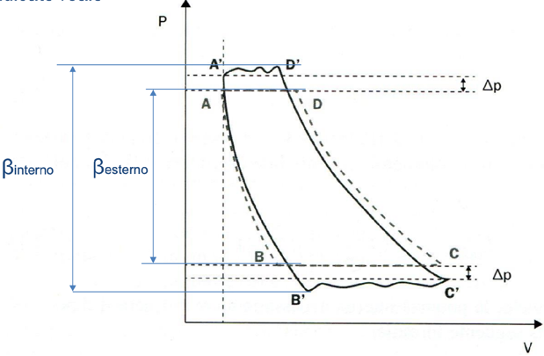
\includegraphics{Immagini/CasoReale.png}
    \caption{Andamento diagramma p-V caso reale}
    \label{fig:CasoReale}
\end{figure}
\\
Partendo da C (C’) come prima, il fluido subisce una compressione per cui la pressione aumenta fino a D’, che si trova a pressione maggiore rispetto ad A. Si nota inoltre che D’ è leggermente più alto rispetto ad A’ perché la valvola rappresenta una perdita di carico concentrata e il fluido attraversandola diminuisce la sua pressione (l’andamento è oscillatorio per motivi legati alla dinamica del gas). \\
Il fluido si ferma ad una pressione leggermente più alta rispetto a quella di mandata (A’-A).\\ Parlando di aria, il moto sarà sicuramente turbolento e le perdite concentrate in tale regime dipendono dal quadrato della velocità del flusso (o dalla portata). La velocità del fluido attraverso la valvola non dipende dalla differenza di pressione (quella è una conseguenza), ma dalla velocità dello stantuffo che spinge fuori il gas.\\
Quindi, le perdite di carico dipendono dalla velocità al quadrato, la velocità dipende dal moto dello stantuffo, quando lo stantuffo va verso il PME, va verso velocità nulla e quindi espelle sempre più lentamente il gas attraverso la valvola, evidenziando perdite di carico sempre più piccole. È per questo che la differenza tra dentro e fuori il cilindro è una differenza che si riduce (andamento decrescente D’-A’). \\
Siccome il  moto del cilindro è molto veloce, nel momento in cui la valvola è aperta non si ha il tempo a sufficienza per uniformare le pressioni tra A’ e A, per cui all’interno del cilindro rimane una pressione più alta della pressione di mandata ($\Delta p_{A'-A}$) da cui inizia direttamente la fase di espansione. \\
\\
Per la fase aspirazione avviene esattamente la stessa cosa, all’interno del cilindro la pressione dovrà essere minore rispetto a quella di aspirazione in modo tale da permettere alla valvola di aprirsi. Durante la fase di ingresso del gas si avrà sempre, all’interno del cilindro, una pressione differente rispetto a quella di aspirazione che va aumentando verso il punto morto inferiore, perché si riduce la velocità di scorrimento dello stantuffo e quindi le perdite di carico. \\
\\
Arrivando al punto C’, appena sotto al punto C, per lo stesso motivo esposto prima, il processo è istantaneo e non c’è tempo per le pressioni di stabilizzarsi. \\
\\
Il diagramma reale, quindi è quello rappresentato in figura, che permette di definire due rapporti di compressione: uno interno ed uno esterno al cilindro.\\
\\
La corsa utile del caso reale si è ridotta rispetto al caso ideale, per cui il coefficiente di riempimento sarà minore rispetto a quello ideale. Le fasi di compressione ed espansione rimangono sostanzialmente delle isoentropiche anche nel ciclo indicato reale. \\
\\
Si capisce immediatamente che mentre il ciclo indicato ideale è definito da delle equazioni che permettono di trovare univocamente i punti di interesse, trovare i punti reali è molto più complicato e i calcoli dovranno essere molto più sofisticati. 
\subsection{Grandezze caratteristiche compressore}

\underline{Dati}: \\
Fluido: aria. \\
Pressione di mandata: $p_M$ = 10 bar.\\
Alesaggio: d = 55 mm.\\
Corsa: s = 42 mm.\\
Cilindrata: $V_d$ = 200 $cm^3$.\\
Velocità di rotazione della manovella: n = 1540 giri/min.\\
Diametro Volano: D = 300 mm ($d_{2m}$= 287 mm). \\
Numero cilindri: N = 2.\\
Stadi di compressione: 1. \\
Per i calcoli si suppone un coefficiente di volume nocivo $\varepsilon$ = 0,05.\\
Essendo il fluido aria il rapporto calore specifico a pressione costante e calore specifico a volume costante è k = 1,4 .\\
Si assume una temperatura di aspirazione pari alla temperatura ambiente T = 293 K (20$^\circ$ C).\\
L’aria può essere considerata “idealmente” come un gas perfetto e pertanto si assumere la costante dei gas R = 287 J/kgK .
\subsubsection{Portata d'aria}
Come descritto nell’introduzione la portata di aria compressa erogata dal compressore è: 
\begin{equation}
    \varepsilon = 0.05.
\end{equation}
\begin{equation}
    \beta=p_M/p_A=11/1=11
\end{equation}
\begin{equation}
    k=1.44
\end{equation}
\begin{equation}
    \lambda_{Vi}=1-\varepsilon\left(\beta^{1/k}-1\right)=0.77
\end{equation}
\begin{equation}
    \rho_{AS}=\frac{p_A}{RT_A}=1.19\ kg/m^3
\end{equation}
\begin{equation}
    \dot{m}=\lambda_{Vi}\cdot\rho_{AS}\cdot\ V_d\cdot\frac{n}{60}=4.7\cdot{10}^{-3}\ kg/m^3
\end{equation}
\subsubsection{Temperatura di mandata}Si può considerare che un gas compresso aumenti la propria temperatura secondo l’equazione dell’isoentropica e di conseguenza nascono alcuni problemi:
\begin{itemize}
    \item Difficoltà nella scelta materiali con cui deve essere realizzato il compressore (tenute stantuffo-cilindro). 
    \item Difficoltà nella lubrificazione (non si possono ammettere particelle di lubrificante in sospensione nel fluido, per questo vengono utilizzati dei segmenti che impongono vincoli sulla temperatura).
\end{itemize}
Questi problemi legati alla temperatura intervengono già da un rapporto di compressione da 5 a 8. Tuttavia, il motivo per il quale il rapporto di compressione del sistema in esame può spingersi fino a 11 è perché, essendo una macchina adibita al settore hobbistico, l’affidabilità richiesta è minore rispetto ad una adibita al settore industriale.\\
\\
Per calcolare la temperatura di mandata si utilizzano le relazioni termodinamiche dell’isoentropica: 
\begin{equation}
    T_M=T_A\ \beta^\frac{k-1}{k}
\end{equation}
sostituendo con i valori, si ottiene $T_M=581,3\ K=308,3^\circ C$.\\
\\
È stato ricavato nell’ambiente di programmazione Matlab l’andamento della temperatura di mandata in funzione del rapporto di compressione $\beta$. 
\begin{figure}[h]
    \centering
    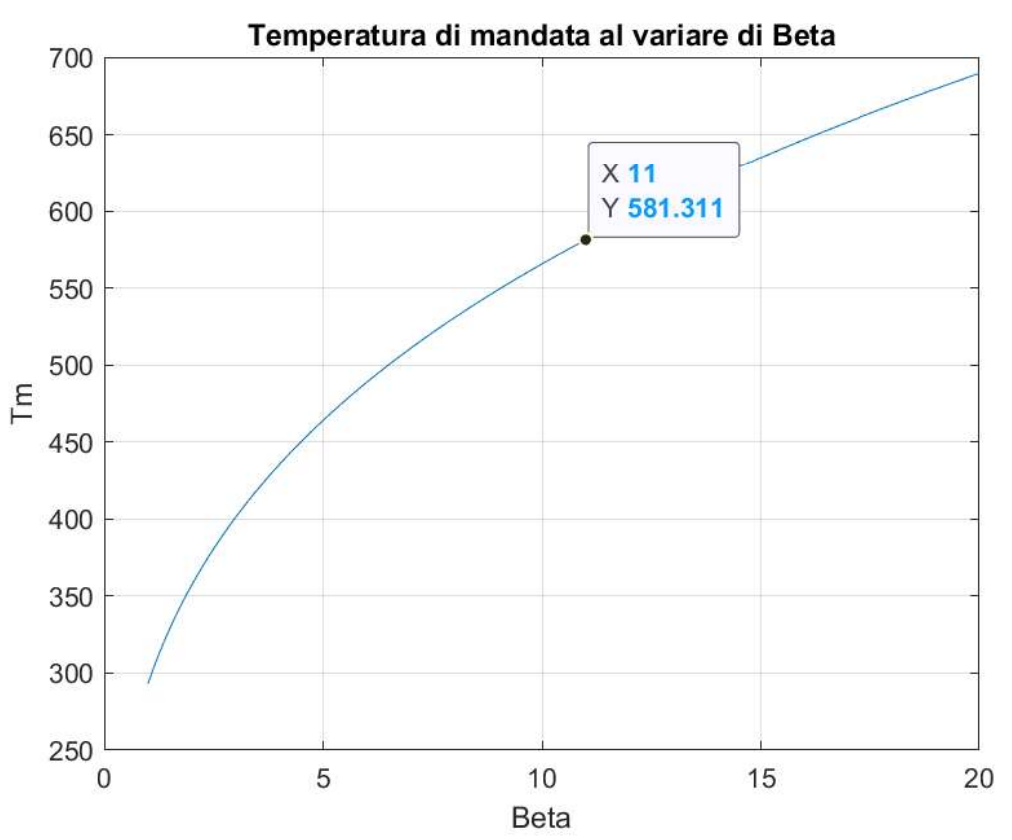
\includegraphics[scale=0.6]{Immagini/GraficoTmBeta.png}
    \caption{Andamento della temperatura di mandata in funzione di $\beta$}
    \label{fig:GraficoTmBeta}
\end{figure}
\\
\\
\begin{lstlisting}[frame=trBL]
%%Dati
Ta=293;                  %Temperatura di aspirazione
k=1.4;                   %Coefficiente isoentropica
eps=0.05;                %Coefficiente volume nocivo
Cil=0.0002;              %Cilindrata[metri cubi]
Pa=101325;               %Pressione Aspirazione[Pa]
Pm=1114575;              %Pressione Mandata[Pa]

%Grafico Temperatura di Mandata%
Beta=1:0.1:20;          %Definizione di beta
Tm=Ta*Beta.^((k-1)/k);  %Calcolo parametro controllato 
plot(Beta,Tm);
xlabel('Beta'),ylabel('Tm'),title('Temperatura di mandata al variare 
      di Beta'),grid on;
\end{lstlisting}
\subsubsection{Diagramma indicato p-V}In conclusione, alla trattazione riguardante l’analisi della macchina, viene di seguito rappresentato il diagramma indicato p-V. \\
Il grafico sarà costituito da 2 trasformazioni isobare, una a $p_M$ e una a $p_A$ e da due isoentropiche, una di espansione e una di compressione. \\
Il ciclo è ottenuto mediante codice all’interno dell’ambiente di programmazione Matlab. 
\begin{figure}[h]
    \centering
    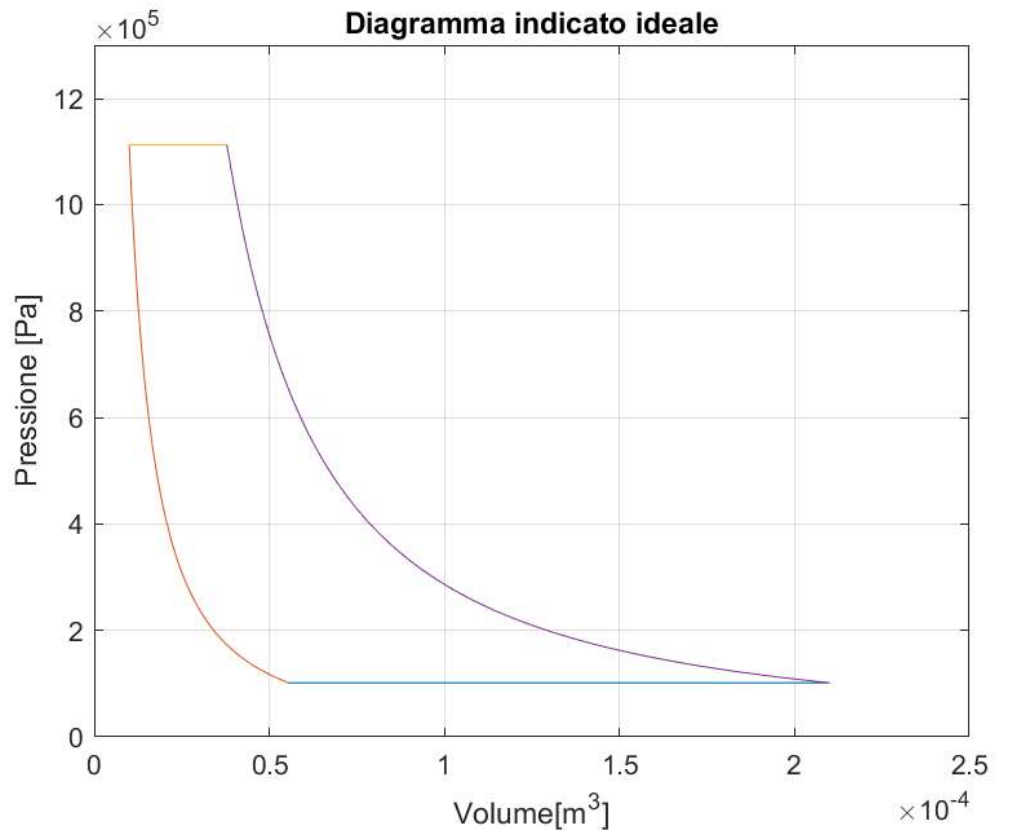
\includegraphics[scale=0.6]{Immagini/GraficopV.png}
    \caption{Andamento diagramma p-V compressore}
    \label{fig:GraficopV}
\end{figure}
\\
\\
\\
\\
\begin{lstlisting}[frame=trBL]
%%Dati
Ta=293.15;              %Temperatura di aspirazione
K=1.4;                  %Coefficiente isentropica
eps=0.05;               %Coefficiente volume nocivo
Cil=0.0002;             %Cilindrata
Pa=101325;               %Pressione Aspirazione
Pm=1114575;              %Pressione Mandata

%%Grandezze Ricavate
Vpmi=Cil*(1+eps);                    %Volume punto morto inferiore
Vpms=Cil*eps;                        %Volume punto morto superiore

%Grafico Ciclo ideale compressore%

%Compressione del fluido
Pciclo=Pa:500:Pm;            %Definizione vettore pressioneda Pa a Pm
Vciclo=(Pa.^(1/K))*(Pciclo.^(-1/K))*Vpmi; %Calcolo Volume 
                                          %in fase di compressione
%Espulsione del fluido
Vespuls=linspace(Vpms,3.79067*10^-5,5);  %Definizione vettore Volume 
                                         %Espulsione
%Espansione
Vcicloesp=(Pm.^(1/K))*(Pciclo.^(-1/K))*Vpms;  %Calcolo Volume 
                                              %Espansione
%Aspirazione
Vaspirato=linspace(5.54437*10^-5,Vpmi,5);  %Definizione vettore Volume 
                                           %Aspirazione
plot(Vaspirato,Pcicloasp);
hold on
plot(Vcicloesp,Pciclo);
hold on 
plot(Vespuls,Pcicloesp);
hold on;
plot(Vciclo,Pciclo);
xlabel('Volume[m^3]'),ylabel('Pressione [Pa]'),title
       ('Diagramma indicato ideale'),ylim([0 13*10^5]),grid on;
\end{lstlisting}

